\documentclass{article}

\usepackage[latin1]{inputenc}
\usepackage[x11names, rgb]{xcolor}
\usepackage{tikz}

% GNUPLOT required
\usepackage{verbatim}

\begin{comment}
:Title: Standard deviation
:Tags: Plots, GNUPLOT, Foreach

A nice illustration of the standard deviation and confidence intervals. 

| Author: Till Tantau
| Source: The `latex-beamer-users`_ mailing list

.. _latex-beamer-users: http://www.nabble.com/plotting-a-normal-distribution-curve-t1891442.html
\end{comment}


\begin{document}
\pagestyle{empty}


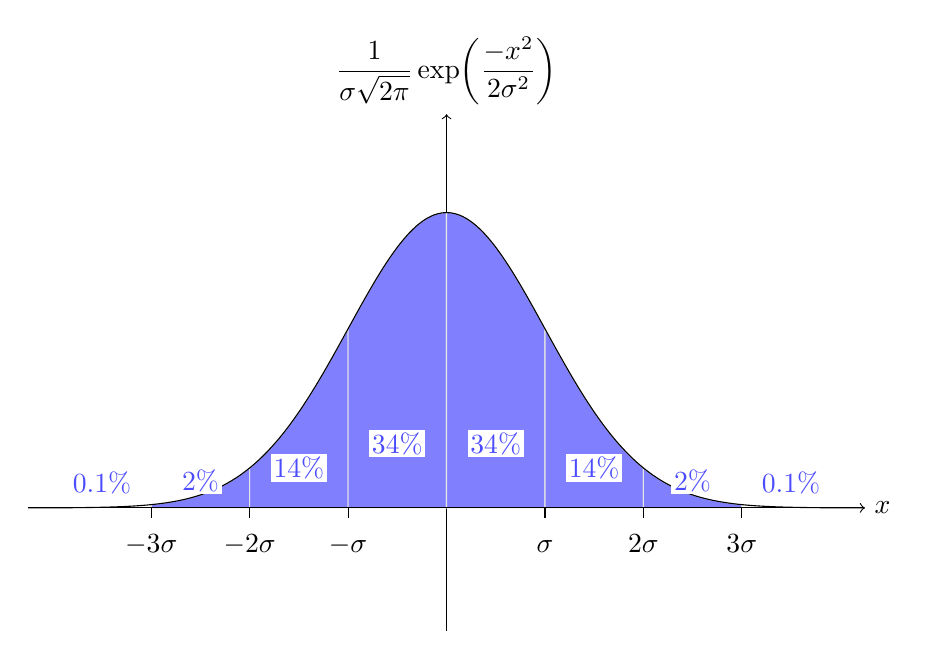
\begin{tikzpicture}[scale=1.25]
    \colorlet{col1}{blue!70}
    \colorlet{col2}{blue!60}
    \colorlet{col3}{blue!50}
    \colorlet{col4}{blue!40}
%   \draw [help lines] (-4.25,-1.25) grid (4.25,1.5);
 %  \draw [help lines,step=0.25cm] (-2.99,0) grid (2.99,0.99);

   \draw[->] (0,-1.25) -- (0,4) node [above]
     {$\displaystyle
        \frac{1}{\sigma\sqrt{2\pi}}\exp\biggl(\frac{-x^2}{2\sigma^2}\biggr)
     $};

   \begin{scope}[smooth,draw=gray!20,y=3cm]
%        \filldraw [fill=col3] plot[id=f1,domain=-3:-2] function {exp(-x*x/2)}
	 \filldraw [fill=col3] plot[id=f1,domain=-3:-2] ({\x},{exp(-\x*\x/2)})
            -- (-2,0) -- (-3,0) -- cycle;
 %       \filldraw [fill=col2] plot[id=f2,domain=-2:-1] function {exp(-x*x/2)}
	 \filldraw [fill=col3] plot[id=f1,domain=-2:-1] ({\x},{exp(-\x*\x/2)})
            -- (-1,0) -- (-2,0) -- cycle;
%        \filldraw [fill=col1] plot[id=f3,domain=-1:0]  function {exp(-x*x/2)}
	 \filldraw [fill=col3] plot[id=f1,domain=-1:0] ({\x},{exp(-\x*\x/2)})
            -- (0,0)  -- (-1,0) -- cycle;
%        \filldraw [fill=col1] plot[id=f4,domain=0:1] function {exp(-x*x/2)}
 	 \filldraw [fill=col3] plot[id=f1,domain=0:1] ({\x},{exp(-\x*\x/2)})
            -- (1,0)  --  (0,0) -- cycle;
  %      \filldraw [fill=col2] plot[id=f5,domain=1:2] function {exp(-x*x/2)}
   	 \filldraw [fill=col3] plot[id=f1,domain=1:2] ({\x},{exp(-\x*\x/2)})
            -- (2,0)  -- (1,0) -- cycle;
%        \filldraw [fill=col3] plot[id=f6,domain=2:3] function {exp(-x*x/2)}
  	 \filldraw [fill=col3] plot[id=f1,domain=2:3] ({\x},{exp(-\x*\x/2)})
            -- (3,0)  -- (2,0) -- cycle;
       \draw[black] plot[id=f7,domain=-4.25:4.25,samples=100]
 %            function {exp(-x*x/2)};
     ({\x},{exp(-\x*\x/2)});
   \end{scope}
       \draw[->] (-4.25,0) -- (4.25,0) node [right] {$x$};

    \foreach \pos/\label in {-3/$-3\sigma$,-2/$-2\sigma$,-1/$-\sigma$,
            1/$\sigma$,2/$2\sigma$,3/$3\sigma$}
        \draw (\pos,0) -- (\pos,-0.1) (\pos cm,-3ex) node
            [anchor=base,fill=white,inner sep=1pt]  {\label};

 %   \draw (-0.1,1) -- (.1,1) node [right,fill=white,inner sep=1pt] {$\sigma$};

    \foreach \pos/\percent/\height in {1/34/0.5,2/14/0.25,3/2/0.125,4/0.1/0.1}
    {
      \node[text=col1,anchor=base,yshift=2pt,xshift=-0.625cm,
        fill=white,inner sep=1pt] at (\pos,\height) {$\percent\%$};
      \node[text=col1,anchor=base,yshift=2pt,xshift=.625cm,
        fill=white,inner sep=1pt]  at (-\pos,\height) {$\percent\%$};
    }
\end{tikzpicture}


\end{document}